\chapter{الانتواع والتطور الكبروي}\label{ch:b2:speciation}

في جزيرة صغيرة من غالاباغوس، سنة 1982، وصلت بضعة عصافير
أرضية كبيرة المناقير من جزيرة مجاورة وبقيت. وطوال
عشرين سنة نافست العصفور الأرضي المتوسط المقيم
على البذور الكبيرة التي يفضلها الاثنان؛ ثم ضرب جفاف، وقلّت
البذور الكبيرة، فجاع المقيمون ذوو المناقير الأكبر ---
أي الذين نافسوا الوافدين أشد منافسة مباشرة.
وفي جيل واحد كانت مناقير المقيمين قد انكمشت، انكماشًا يُقاس،
بعيدًا عن مناقير الغزاة. فنوعان التقيا دُفعا
متباعدين. وهذا الفصل في صنع الأنواع: ما النوع
وما الذي يبقيه متميزًا، وكيف تصير جمهرة واحدة اثنتين،
والمنافسة التي تباعد بين الجمهرات حين تلتقي، و
النظرة الطويلة إلى السجل الأحفوري، حيث يعطي تكرار العملية نفسها
مئة مليون مرة شجرة الحياة.

\section{ما النوع}

\begin{definition}[النوع]\label{def:b2:speciation:species}
\index{مفهوم النوع}\index{مفهوم النوع الحيوي}\index{عزل تكاثري}
بحسب \emph{مفهوم النوع الحيوي}، النوع مجموعة
من الجمهرات يستطيع أفرادها التزاوج فيما بينهم و
إنتاج خلف خصب، ويكونون \emph{معزولين تكاثريًا}
عن المجموعات الأخرى من هذا القبيل: فالذي يوحّد النوع هو \omterm{prop:b2:population-genetics:migration}{التدفق المورّثي}،
والذي يفصل الأنواع هو غيابه. والمفهوم يعمل في
الكائنات الجنسية في زمان ومكان واحد، وهي معظم ما يلقاه
عالم الأحياء؛ ويخفق في السلالات اللاجنسية (التي تُسمى
بالتشابه)، وفي الأحافير (التي لا تُهجَّن)، وفي
الحالات الكثيرة التي تكون فيها الحدود مسربة --- كالبلوط والصفصاف اللذين
يتهجنان عبر الأنواع، والبط الذي تتزاوج أنواعه في
الأسر، والأنواع الحلقية التي تتزاوج فيها الجمهرات المتجاورة
على امتداد الطريق كله حول حاجز حتى يلتقي الطرفان فلا
يتزاوجان. وتملأ مفاهيم أخرى الثغرات: النوع \emph{الشكلي}
(أي عنقود من الأشكال المتشابهة)، و\emph{النشوئي} (أي أصغر
سلالة قابلة للتشخيص)، و\emph{البيئي} (أي سلالة تشغل
مكانتها الخاصة). وليس أي منها خطأ؛ فكل منها يقيس شيئًا حقيقيًا، و
الانتواع هو العملية التي تتفق بها في النهاية.
\end{definition}

\begin{proposition}[آليات العزل]\label{prop:b2:speciation:isolation}
\index{آلية عزل}\index{عزل قبل اللاقحة}\index{عزل بعد اللاقحة}\index{قاعدة هالدين}
\omterm{prop:b2:population-genetics:migration}{التدفق المورّثي} بين جمهرتين توقفه حواجز تفعل
قبل الإلقاح أو بعده. فالعزل \emph{قبل اللاقحة}: تعيش الجمهرتان
في موائل مختلفة أو تتكاثران في مواسم مختلفة (وهو العزل
الزماني: ضفدعان ينقّان في شهرين مختلفين)؛ أو لا
تتعرف إحداهما مغازلة الأخرى (وهو السلوكي: أغاني
صراصير الليل، ورموز ضوء اليراعات، ورقصات البط)؛ أو لا تتلاءم
أعضاؤها التناسلية أو أزهارها (وهو الميكانيكي)؛ أو لا تندمج أعراسها
(وهو العرسي: بروتينات ارتباط النطاف في قنافذ البحر، وأليلات
$S$ في \cref{ch:b2:angiosperm-reproduction}).
والعزل \emph{بعد اللاقحة}: يموت الهجين جنينًا، أو يعيش لكنه
عقيم (البغل؛ وهجائن نوعين من \emph{Drosophila})، أو
يكون خصبًا لكن خلفه ليس كذلك (وهو انهيار الهجين).
و\emph{\omterm{prop:b2:speciation:isolation}{قاعدة هالدين}}: حين يكون جنس واحد من الهجين عقيمًا أو
غير قابل للحياة، كان هو الجنس ذا الصبغيين الجنسيين المختلفين ---
أي الذكر في الثدييات والذباب، والأنثى في الطيور والفراشات ---
لأن عدم التوافق المتنحي على الصبغي X يُكشف فيه.
والحواجز قبل اللاقحة أرخص، إذ لا تُهدر أعراس،
والانتقاء يبنيها حيث توجد حواجز بعد اللاقحة أصلًا.
\end{proposition}

\begin{theorem}[لماذا تخفق الهجائن: نموذج الموقعين]\label{thm:b2:speciation:dm}
\index{عدم توافق دوبجانسكي--مولر}
تبدأ جمهرتان \omterm{def:b2:meiosis-heredity:vocabulary}{بنمط وراثي} $aabb$. ففي إحداهما يتحول $a$
إلى $A$؛ وفي الأخرى يتحول $b$ إلى $B$؛ وكل استبدال محايد أو
مفيد في خلفيته هو، فلا تمر أي جمهرة قط
بحالة أقل \omterm{def:b2:population-genetics:fitness}{لياقة}. لكن $A$ و$B$ لم يُختبرا معًا
قط، وإن كان الاجتماع غير متوافق --- أي إن كان البروتين
الذي يصنعه $A$ لا يعمل مع البروتين الذي يصنعه $B$ --- كان
الهجين $AaBb$ غير لائق. فينشأ \omterm{def:b2:speciation:species}{العزل التكاثري} إذن ناتجًا
عرضيًا للتباعد، دون عبور أي وادٍ ودون انتقاء
للعزل نفسه؛ ولأن كل استبدال جديد في سلالة
قد لا يتوافق مع كل استبدال مثبَّت أصلًا
في الأخرى، ينمو عدد حالات عدم التوافق الممكنة على صورة \emph{مربع}
عدد الاستبدالات --- فالعزل \emph{يتكوّر ككرة الثلج}
مع الزمن.
\end{theorem}
\begin{proof}
مع $n$ استبدالًا في كل سلالة، قد لا يتوافق كل من الأليلات $n$
الجديدة في سلالة مع كل من الأليلات $n$ في
الأخرى: أي $n^{2}$ زوج، كل منها غير متوافق باحتمال
$\varepsilon$، فيكون عدد حالات عدم التوافق المنتظر
$\varepsilon n^{2}$، وينمو $n$ مع الزمن منذ الانفصال.
والهجين هو \omterm{def:b2:meiosis-heredity:vocabulary}{النمط الوراثي} الوحيد الذي تلتقي فيه المجموعتان.
\end{proof}
\begin{proof}[شواهد]
جمع كوين وأور (1989 و1997) مئات أزواج أنواع
\emph{Drosophila} معلومة المسافة الوراثية (وهي مقياس
للزمن منذ التباعد) وقاسا عزلها قبل اللاقحة
وبعدها: فكلاهما يرتفع مع المسافة، والعزل
يكاد يكتمل عند مسافة توافق بضعة ملايين من
السنين، والأزواج التي تعيش في المنطقة نفسها تظهر عزلًا
أقوى قبل اللاقحة عند مسافة معطاة من الأزواج التي لا تعيش كذلك ---
وهو توقيع التعزيز. وقد عُرّفت مورّثات عدم التوافق منذ ذلك الحين
واحدة واحدة، وعدد ما يوجد منها بين نوعين
ينمو فعلًا أسرع من النمو الخطي مع تباعدهما.
\end{proof}

\begin{omfigure}
\begin{tikzpicture}[every node/.style={font=\scriptsize}, >=stealth]
  \node[draw, rounded corners, fill=omExo!25] (anc) at (0,0) {السلف $aabb$};
  \node[draw, rounded corners, fill=omDef!15] (p1) at (-2.6,-1.8) {الجمهرة 1: $AAbb$};
  \node[draw, rounded corners, fill=omThm!15] (p2) at (2.6,-1.8) {الجمهرة 2: $aaBB$};
  \node[draw, rounded corners, fill=gray!25, align=center] (hyb) at (0,-3.6) {الهجين $AaBb$:\\يلتقي $A$ و$B$ أول مرة\\--- غير متوافقين وغير لائقين};
  \draw[->, thick] (anc) -- (p1) node[midway, left, align=right] {تثبيت $a \to A$،\\لائق في خلفيته};
  \draw[->, thick] (anc) -- (p2) node[midway, right, align=left] {تثبيت $b \to B$،\\لائق في خلفيته};
  \draw[->, thick] (p1) -- (hyb); \draw[->, thick] (p2) -- (hyb);
  \node[anchor=west, align=left, text width=4.6cm] at (4.6,-0.4) {لم تعبر أي جمهرة واديًا؛ فالعزل ناتج عرضي، وعدد هذه الأزواج ينمو على صورة $n^{2}$};
\end{tikzpicture}

{\small نموذج الموقعين لإخفاق الهجين. تثبت كل جمهرة
تغيرًا يعمل في خلفيتها هي؛ والهجين أول
\omterm{def:b2:meiosis-heredity:vocabulary}{نمط وراثي} يجمع الاثنين.}
\end{omfigure}

\section{كيف يصير نوع واحد نوعين}

\begin{proposition}[أنماط الانتواع]\label{prop:b2:speciation:modes}
\index{انتواع جغرافي}\index{انتواع متشارك المكان}\index{انتواع متجاور}\index{أثر المؤسس}
\emph{\omterm{prop:b2:speciation:modes}{الانتواع الجغرافي}} يبدأ بحاجز جغرافي:
مدى يشقه جبل ناهض، أو بحر يجف، أو نهر جديد
(وهو \emph{الانشطار المكاني})، أو بضعة مستعمرين يُحملون إلى جزيرة
(وهو \emph{الانتواع المحيطي}، ومعه \omterm{prop:b2:speciation:modes}{أثر المؤسس} والانجراف في
\cref{ch:b2:population-genetics}). فإذ تُقطع الجمهرتان عن \omterm{prop:b2:population-genetics:migration}{التدفق المورّثي}
تتباعدان بالانتقاء في بيئتين مختلفتين،
وبالانجراف، وبطفراتهما المنفصلة، حتى تتراكم حالات عدم التوافق؛
فإذا التقتا من جديد لم تعودا تندمجان. وهو
أشيع الأنماط، ونمط الأنواع الشقيقة على جهتي
كل برزخ وسلسلة جبال ومضيق سجلُّه.
أما \emph{\omterm{prop:b2:speciation:modes}{الانتواع المتشارك المكان}} فيحدث بلا حاجز: إما في خطوة واحدة
بتعدد الصيغ (\cref{ch:b2:genome-diversification}) --- وقد نشأ ثلث
أنواع النبات هكذا؛ وإما بانتقاء مفرِّق مع تزاوج
انتقائي، حين تستغل جمهرة موردين ويتزاوج
الأفراد على المورد الذي يستعملونه (كذبابة يرقة التفاح
التي انتقلت من الزعرور إلى التفاح في ستينيات القرن التاسع عشر وتتزاوج الآن على
عائلها؛ وبلطيات بحيرة فوهية). و\emph{\omterm{prop:b2:speciation:modes}{الانتواع المتجاور}}
يحدث على امتداد تدرج بيئي، حيث تتكيف
جمهرة مع الطرفين وتتشكل \omterm{prop:b2:speciation:reinforcement}{منطقة تهجين} في
الوسط. والوصفة في كل الأنماط واحدة: قلّل \omterm{prop:b2:population-genetics:migration}{التدفق المورّثي}،
ودع التباعد يتراكم، ودع النواتج العرضية للتباعد
تصير حواجز.
\end{proposition}

\begin{omfigure}
\resizebox{\linewidth}{!}{%
\begin{tikzpicture}[every node/.style={font=\scriptsize}, >=stealth]
  \foreach \x/\lab in {0/{جغرافي:\\حاجز يشق المدى}, 5.2/{محيطي:\\بضعة مؤسسين على جزيرة}, 10.4/{متشارك المكان:\\عائلان والتزاوج على العائل}} \node[align=center, anchor=south] at (\x+1.8,3.0) {\lab};
  % allopatric
  \draw[thick, fill=omDef!15] (0.9,1.4) ellipse (0.8 and 0.9);
  \draw[thick, fill=omThm!15] (2.7,1.4) ellipse (0.8 and 0.9);
  \draw[very thick, omExo!70!black] (1.8,0.2) -- (1.8,2.6);
  \node[below] at (1.8,0.1) {جبل أو بحر أو نهر};
  % peripatric
  \begin{scope}[xshift=5.2cm]
    \draw[thick, fill=omDef!15] (1.0,1.4) ellipse (1.0 and 0.9);
    \draw[thick, fill=omThm!15] (3.2,1.9) circle (0.35);
    \draw[->, thick, dashed] (2.0,1.6) -- (2.85,1.85);
    \node[below] at (3.2,1.5) {مؤسسون};
    \node[below] at (1.0,0.4) {بر رئيس};
  \end{scope}
  % sympatric
  \begin{scope}[xshift=10.4cm]
    \draw[thick, fill=omExo!15] (1.8,1.4) ellipse (1.7 and 0.9);
    \foreach \p in {(1.0,1.6),(1.3,1.2),(0.8,1.2),(1.2,1.8)} \fill[omDef] \p circle (0.07);
    \foreach \p in {(2.4,1.6),(2.7,1.2),(2.2,1.2),(2.6,1.8)} \fill[omThm] \p circle (0.07);
    \node[omDef, below] at (1.0,0.5) {العائل A}; \node[omThm, below] at (2.6,0.5) {العائل B};
    \node[below] at (1.8,0.1) {مكان واحد ومورَدان};
  \end{scope}
\end{tikzpicture}}

{\small ثلاث طرق إلى نوعين: حاجز يشق المدى، أو
جمهرة مؤسِّسة وراءه، أو مورَدان داخله.}
\end{omfigure}

\begin{proposition}[التعزيز ومناطق التهجين]\label{prop:b2:speciation:reinforcement}
\index{تعزيز}\index{منطقة تهجين}\index{تدرج جغرافي}
حين تلتقي جمهرتان متباعدتان من جديد، يمكن أن يحدث ثلاثة أمور.
فإن كانت هجائنهما لائقة كالآباء اندمجتا. وإن كانت
الهجائن غير لائقة حبّذ الانتقاء الأفراد الذين يأبون
التزاوج مع الصنف الآخر --- والأعراس المهدرة هي الكلفة ---
وقوي \omterm{prop:b2:speciation:isolation}{العزل قبل اللاقحة} حيث يتداخل الاثنان
(وهو \emph{التعزيز})، حتى يصيرا نوعين. وبين هاتين الحالتين تدوم
\emph{\omterm{prop:b2:speciation:reinforcement}{منطقة تهجين}}: أي شريط عرضه بضعة كيلومترات في الغالب،
يتزاوج فيه الشكلان وتُنتج الهجائن في كل
جيل، ويبقيه ميزان الانتشار إلى داخل
المنطقة والانتقاء ضد الهجائن داخلها. وعبر تلك
المنطقة يتبع تواتر كل شكل \emph{تدرجًا جغرافيًا}، أي منحنيًا
على شكل حرف S عرضه $w$ تقرره مسافة الانتشار $\sigma$ في
الجيل والانتقاء $s$ ضد الهجائن، $w \approx
\sigma\sqrt{8/s}$: فالمنطقة قد تبقى ضيقة آلاف السنين
دون أن يندمج الشكلان أو ينفصلا تمامًا. وضفادع
أوروبا وغربانها وفئرانها وجنادبها تُظهر عشرات منها، معظمها
يجري على امتداد الخطوط التي التقت عندها من جديد الجمهرات التي احتمت في
ملاجئ منفصلة خلال العصر الجليدي الأخير إذ انسحب الجليد.
\end{proposition}
\begin{proof}[شواهد]
حيث يتداخل الخاطف المُبَرقع والخاطف المطوَّق في وسط أوروبا،
يكون ريش ذكور كل نوع أشد اختلافًا عن ريش
الآخر مما هو حيث يعيشان متفرقين، وتميّز الإناث تمييزًا
أحد --- أي تعزيز مقيس في الحقل. وتلتقي علاجيم البطن النارية
والبطن الصفراء على امتداد منطقة تعبر بولندا عرضها بضعة
كيلومترات، ثابتة ما دامت قد دُرست، ويُتنبأ
بعرض تدرجها من انتشارها ومن انخفاض
\omterm{def:b2:population-genetics:fitness}{لياقة} هجائنها.
\end{proof}

\begin{omfigure}
\begin{tikzpicture}
\begin{axis}[
  width=0.72\linewidth, height=5.2cm,
  axis x line=bottom, axis y line=left,
  xmin=-30, xmax=30, ymin=0, ymax=1.05,
  xlabel={المسافة عبر المنطقة (km)}, ylabel={تواتر الشكل A},
  xlabel style={font=\small, at={(axis description cs:0.5,-0.13)}, anchor=north},
  ylabel style={font=\small},
  tick label style={font=\small}, xtick={-20,-10,0,10,20}, ytick={0,0.5,1},
  clip=false,
]
\addplot[very thick, omDef, domain=-30:30, samples=100] {1/(1+exp(x/2.2))};
\draw[dashed, gray] (axis cs:-4.4,0) -- (axis cs:-4.4,1); \draw[dashed, gray] (axis cs:4.4,0) -- (axis cs:4.4,1);
\draw[<->] (axis cs:-4.4,0.08) -- (axis cs:4.4,0.08); \node[font=\scriptsize, anchor=south] at (axis cs:0,0.09) {العرض $w$};
\node[font=\scriptsize, anchor=west, align=left] at (axis cs:8,0.75) {$w \approx \sigma\sqrt{8/s}$: انتشار\\$\sigma = \qty{1}{km}$، $s = 0.1$\\يعطيان $w \approx \qty{9}{km}$};
\end{axis}
\end{tikzpicture}

{\small \omterm{prop:b2:speciation:reinforcement}{تدرج جغرافي} عبر \omterm{prop:b2:speciation:reinforcement}{منطقة تهجين}: تواتر أحد الشكلين
يهبط من واحد إلى صفر على عرض يقرره كم ينتشر الأفراد
وكم هجائنهم غير لائقة.}
\end{omfigure}

\section{المنافسة والتعايش وإزاحة الصفات}

\begin{theorem}[منافسة لوتكا--فولتيرا]\label{thm:b2:speciation:lv}
\index{منافسة لوتكا--فولتيرا}\index{إقصاء تنافسي}\index{تعايش}
نوعان ينموان نموًا لوجستيًا (كما في مجلد السنة الأولى) ويتنافسان
على مورد يخضعان للمعادلتين
\[
\frac{\mathrm{d}N_1}{\mathrm{d}t} = r_1 N_1\Bigl(1 - \frac{N_1 + \alpha N_2}{K_1}\Bigr), \qquad
\frac{\mathrm{d}N_2}{\mathrm{d}t} = r_2 N_2\Bigl(1 - \frac{N_2 + \beta N_1}{K_2}\Bigr),
\]
حيث يقيس $\alpha$ أثر فرد واحد من النوع 2
في النوع 1 بوحدات أفراد النوع 1 نفسه، ويقيس $\beta$
العكس. ويكف النوع 1 عن النمو على الخط $N_1 + \alpha N_2 =
K_1$ (وهو \emph{خط تساويه})، ويكف النوع 2 على $N_2 + \beta N_1 = K_2$،
وتتوقف الحصيلة على كيفية تقاطع الخطين:
\begin{itemize}
  \item $K_1 > \alpha K_2$ و$K_2 < \beta K_1$: يفوز النوع 1
        دائمًا؛
  \item $K_1 < \alpha K_2$ و$K_2 > \beta K_1$: يفوز النوع 2
        دائمًا؛
  \item $K_1 > \alpha K_2$ و$K_2 > \beta K_1$: \emph{تعايش
        مستقر} عند $N_1^{*} = (K_1 - \alpha K_2)/(1 - \alpha\beta)$
        و$N_2^{*} = (K_2 - \beta K_1)/(1 - \alpha\beta)$؛
  \item $K_1 < \alpha K_2$ و$K_2 < \beta K_1$: يفوز أيهما،
        بحسب من يبدأ أكثر عددًا.
\end{itemize}
ويقتضي التعايش $\alpha\beta < 1$ مع كون كل نوع يكبحه
بنو جنسه أكثر مما يكبحه الآخر: فنوعان يستعملان
المورد نفسه بالضبط ($\alpha = \beta = 1$) لا يستطيعان التعايش
(وهو \emph{مبدأ \omterm{thm:b2:speciation:lv}{الإقصاء التنافسي}})، وكلما زاد
اختلاف ما يستعملانه صغر $\alpha$ و$\beta$ وكان
تعايشهما أوثق.
\end{theorem}
\begin{proof}
على خط تساوي النوع 1 يكون $\mathrm{d}N_1/\mathrm{d}t = 0$؛ وتحته
(نحو المبدأ) ينمو $N_1$، وفوقه يهبط $N_1$؛ وكذلك
النوع 2. وكل خط تساوٍ مستقيم تقاطعاته $K_1$
على محور $N_1$ و$K_1/\alpha$ على محور $N_2$ (للنوع 1)،
و$K_2/\beta$ و$K_2$ (للنوع 2). ويستطيع النوع 1 غزو
جمهرة من النوع 2 عند حمولتها القصوى $K_2$ إن كان نموه
هو موجبًا هناك، أي إن كان $K_1 > \alpha K_2$؛ ويستطيع النوع 2
غزو النوع 1 عند $K_1$ إن كان $K_2 > \beta K_1$. وحين يستطيع كل منهما غزو
الآخر لا يمكن إقصاء أي منهما وتتقارب المسارات إلى
تقاطع خطي التساوي، ويُوجد بحل معادلتي المستقيمين؛
وحين لا يستطيع إلا أحدهما، فاز؛ وحين لا يستطيع أي منهما، كان
التقاطع سرجًا وفاز المؤسس. واستقرار النقطة الداخلية
يتبع من حجة الغزو: فإذا اضطربت نحو أي من
المحورين نما النوع الأندر من جديد.
\end{proof}

\begin{omfigure}
\begin{tikzpicture}
\begin{axis}[
  width=0.6\linewidth, height=6cm,
  axis x line=bottom, axis y line=left,
  xmin=0, xmax=1300, ymin=0, ymax=1900,
  xlabel={$N_1$}, ylabel={$N_2$},
  xlabel style={font=\small, at={(axis description cs:0.5,-0.1)}, anchor=north},
  ylabel style={font=\small},
  tick label style={font=\small}, xtick={0,857,1000,1333}, xticklabels={0,$N_1^*$,$K_1$,$K_2/\beta$}, ytick={0,286,800,2000}, yticklabels={0,$N_2^*$,$K_2$,$K_1/\alpha$},
  clip=false,
]
\addplot[very thick, omDef, domain=50:1000, samples=2] {(1000-x)/0.5};
\addplot[very thick, omThm, domain=0:1333, samples=2] {800-0.6*x};
\fill[black] (axis cs:857,286) circle (2.5pt);
\draw[->, thick, gray] (axis cs:150,1750) -- (axis cs:300,1450);
\draw[->, thick, gray] (axis cs:1200,100) -- (axis cs:1000,250);
\draw[->, thick, gray] (axis cs:150,150) -- (axis cs:400,250);
\node[font=\scriptsize, omDef, anchor=west] at (axis cs:700,1000) {خط تساوي النوع 1};
\node[font=\scriptsize, omThm, anchor=south west] at (axis cs:130,740) {خط تساوي النوع 2};
\node[font=\scriptsize, anchor=south west] at (axis cs:880,320) {تعايش مستقر};
\end{axis}
\end{tikzpicture}

{\small مستوي الطور لمتنافسين عند $K_1 = 1000$ و$K_2 =
800$ و$\alpha = 0.5$ و$\beta = 0.6$: يستطيع كل نوع غزو
الحمولة القصوى للآخر، وتتقارب المسارات على
تقاطع خطي التساوي عند $N_1^{*} = 857$ و$N_2^{*} = 286$.}
\end{omfigure}

\begin{proposition}[إزاحة الصفات]\label{prop:b2:speciation:displacement}
\index{إزاحة الصفات}\index{مكانة}\index{إشعاع تكيفي}
المنافسة ليست حصيلة بيئية فحسب بل قوة
تطورية. فحيث يلتقي نوعان متشابهان، يعاني من المنافسة أشد المعاناة
أفرادُ كل منهما الأشبه بالآخر،
ويدفع الانتقاء الاثنين متباعدين في الصفة التي تحكم
استعمال المورد --- كحجم المنقار أو حجم الجسم أو وقت الإزهار: فتختلف
الجمهرات المتداخلة أكثر مما تختلف الجمهرات التي تعيش
وحدها. وهذه \emph{\omterm{prop:b2:speciation:displacement}{إزاحة الصفات}} تصغّر $\alpha$
و$\beta$، وتحوّل صراعًا على الإقصاء إلى تعايش، وهي، إذ
تتكرر عبر مشهد من الفرص، تنتج
\emph{إشعاعًا تكيفيًا}: أي مستعمرًا واحدًا يصير عشرات الأنواع
ملائم كل منها لمورد --- كعصافير داروين في غالاباغوس،
وطيور العسل في هاواي، وبلطيات البحيرات الإفريقية
(خمسمئة نوع في بحيرة فكتوريا في أقل من خمسة عشر ألف
سنة)، وسحالي الأنول في الكاريبي، حيث ملأت المجموعةَ نفسها من
المكانات المجموعةُ نفسها من أشكال الجسم استقلالًا
في أربع جزر.
\end{proposition}
\begin{proof}[شواهد]
سجّل الزوجان غرانت كل عصفور في دافني ميجور أربعين سنة.
وبعد أن استقر العصفور الأرضي الكبير سنة 1982، لم يتغير
منقار العصفور الأرضي المتوسط حتى جفاف
سنة 2004، حين ندرت البذور الكبيرة وتنافس النوعان
عليها؛ فمات ذوو المناقير الأكبر من العصافير المتوسطة
بنسبة غير متناسبة، وكانت مناقير الجيل التالي أصغر بأكثر
مما رُئي قط في خطوة واحدة --- أي \omterm{prop:b2:speciation:displacement}{إزاحة الصفات}
التي تنبأت بها النظرية، ملحوظةً وهي تحدث، مع
قياس فرق انتقائها وقابلية توريثها. وأظهرت مناقير العصافير
نفسها، بمقارنتها بين جزر تعيش فيها وحدها وجزر
تلتقي فيها، الإزاحة نفسها مكتوبةً عبر
الأرخبيل.
\end{proof}

\begin{omfigure}
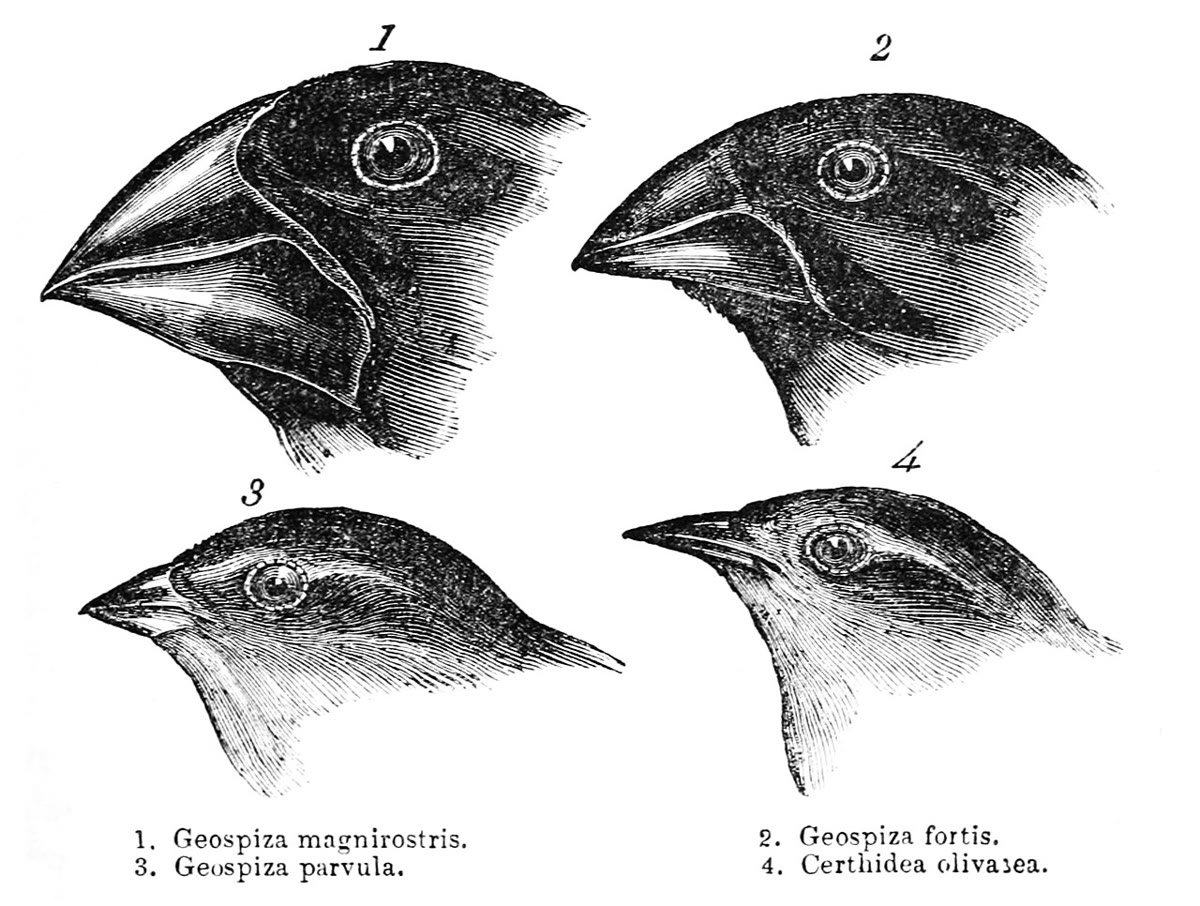
\includegraphics[width=0.44\linewidth]{images/book2/finches-gould.jpg}\hspace{0.04\linewidth}
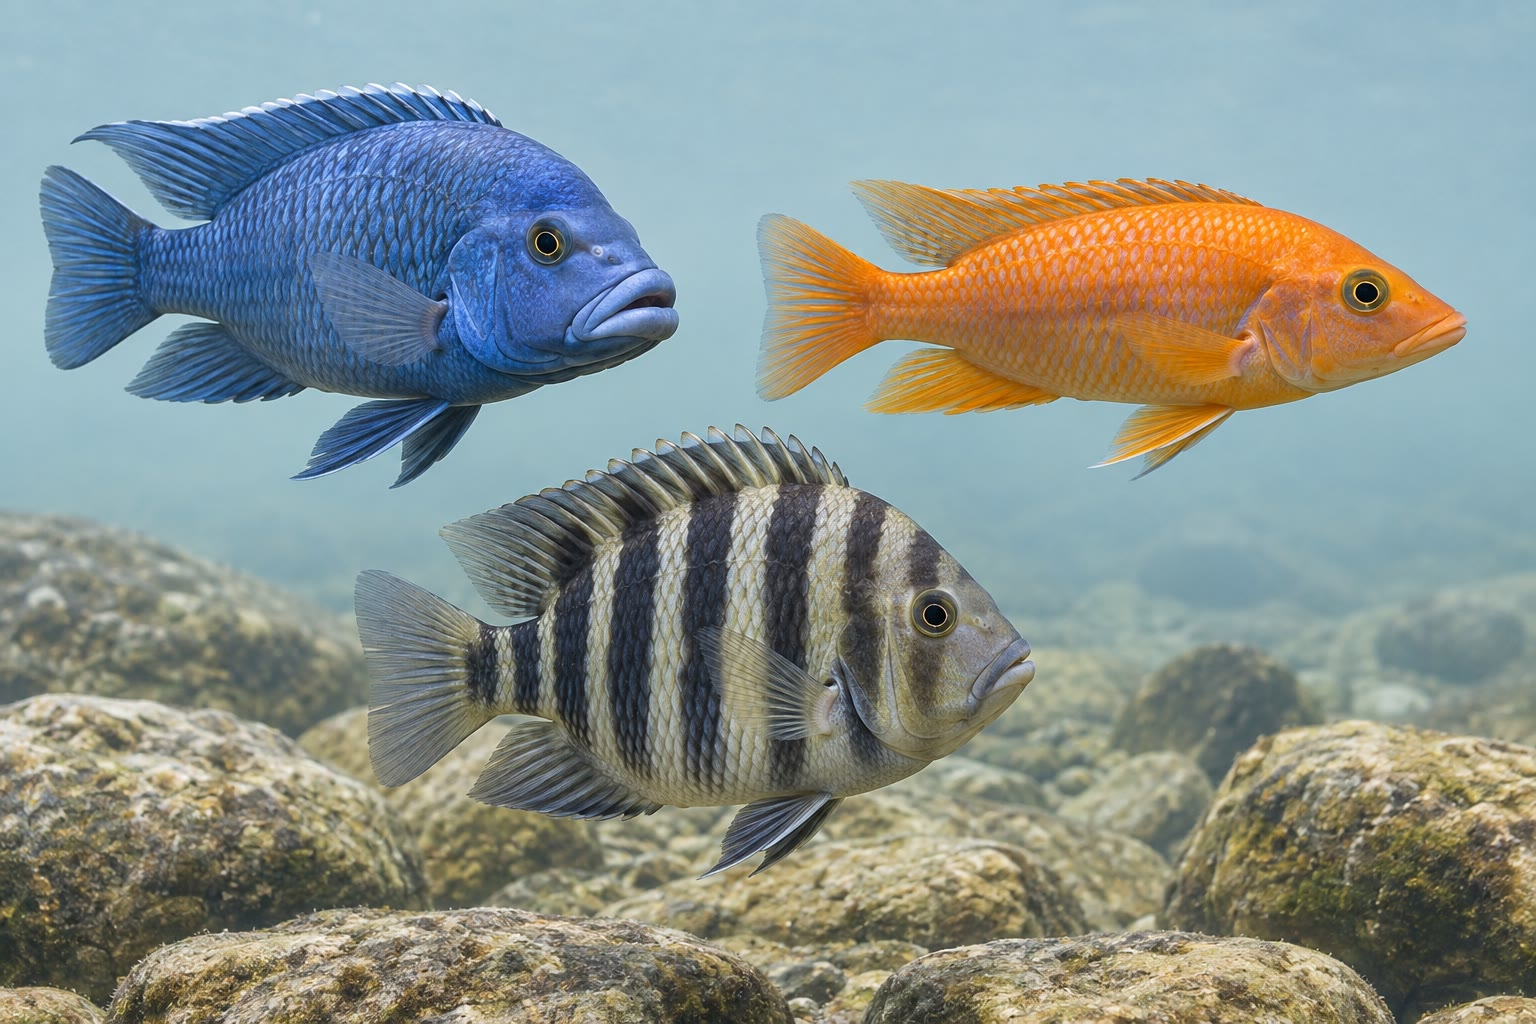
\includegraphics[width=0.44\linewidth]{images/book4/ai/b4-23-cichlids.jpg}

{\small إشعاعان. إلى اليسار: عصافير داروين كما رسمها غولد سنة
1845، مستعمر واحد صار كثيرين، تميزها مناقيرها.
وإلى اليمين: بلطيات بحيرة إفريقية، مئات الأنواع من بضعة
مؤسسين، لكل منها فمه وغذاؤه.}
\end{omfigure}

\section{التطور الكبروي: النظرة الطويلة}

\begin{proposition}[الإيقاع والنمط]\label{prop:b2:speciation:tempo}
\index{توازن متقطع}\index{تدرجية}\index{انقراض جماعي}
على مدى بضعة عشرات من الأجيال غيّرت الفراشة لونها وغيّر العصفور
منقاره؛ وعلى مدى ملايين السنين يُظهر السجل الأحفوري سلالات
لا تكاد تتغير في فترات طويلة ثم، في
لحظة جيولوجية طولها بضعة آلاف من السنين، يحل محلها سليل
متميز --- وهو \emph{\omterm{prop:b2:speciation:tempo}{التوازن المتقطع}}، وهو ما يبدو عليه
\omterm{prop:b2:speciation:modes}{الانتواع الجغرافي} في جمهرات طرفية صغيرة يتلوه
انتشارها حين تُؤخذ العينات كل مئة ألف سنة؛
ويُظهر السجل سلالات أخرى، منها الخيول، تتغير
تدرجيًا عبر عشرات الأنواع. وفوق النوع يكون السجل
سجل تبدّل: فمعظم الأنواع تدوم من مليون إلى عشرة ملايين سنة،
ومعدل \emph{الانقراض الخلفي} نحو نوع واحد من
مليون في السنة، وخمس مرات --- في نهاية الأوردوفيشي
والديفوني والبرمي (حين زالت تسعة أعشار الأنواع البحرية)
والترياسي والطباشيري --- أزال \emph{\omterm{prop:b2:speciation:tempo}{انقراض جماعي}} معظم
ما كان حيًّا في غضون بضع مئات الآلاف من السنين وأعاد ضبط اللعبة،
فأشعّت الناجيات في المكانات الخالية: كالثدييات في
عالم الديناصورات بعد كويكب قبل 66 مليون سنة.
فالتطور الكبروي هو النمط الذي رسمه التطور الصغروي في هذا
الفصل والفصل السابق، إذا أُجري زمنًا طويلًا جدًا وقاطعته
كارثة.
\end{proposition}

\begin{example}[مقارنة المعدلات]\label{ex:b2:speciation:rates}
غيّر الانتقاء على العصافير عمق المنقار بمقدار \qty{4}{\%} في جيل
واحد؛ واستغرق إشعاع غالاباغوس كله، بأربعة عشر نوعًا من
مؤسس واحد، مليوني سنة؛ والفرق بين فأر
وفيل في حجم الجسم، وهو نحو $10^{5}$، كان يمكن أن ينتجه
انتقاء بقوة انتقاء العصافير في بضع مئات من الأجيال ---
ومع ذلك يبيّن السجل أنه استغرق أربعين مليون سنة. ويُحل التناقض
بملاحظة أن الانتقاء نادرًا ما يدفع في الاتجاه نفسه
طويلًا: فهو ينقلب مع الطقس، كما انقلب في دافني ميجور في
السنة التالية للجفاف، \omterm{prop:b2:population-genetics:kinds}{والانتقاء المثبِّت} يبقي معظم
السلالات حيث هي. فالتغير المستدام نادر، ولذلك كان
الانتواع، وهو يحتاجه، بطيئًا --- ولذلك، حين يتغير العالم
سريعًا، كما يفعل في \cref{ch:b2:global-change}، تضيع
السلالات التي لا تستطيع اللحاق.
\end{example}

\section{تمارين}

\begin{exercise}[$\star$]\label{exo:b2:speciation:1}
اذكر \omterm{def:b2:speciation:species}{مفهوم النوع الحيوي} وأعطِ ثلاث حالات لا
يمكن تطبيقه فيها، مع المفهوم المستعمل بدلًا منه.
\end{exercise}

\begin{exercise}[$\star$]\label{exo:b2:speciation:2}
صنّف ما يلي عزلًا قبل اللاقحة أو بعدها: ضفدعان يتكاثران في
شهرين مختلفين؛ وبغل؛ ونطفة قنفذ بحر لا تستطيع الارتباط
ببيضة نوع آخر؛ ونباتات هجينة عافية لكن
بذورها لا تنبت؛ وصرصارا ليل بأغنيتين مختلفتين.
\end{exercise}

\begin{exercise}[$\star$]\label{exo:b2:speciation:3}
عرّف \omterm{prop:b2:speciation:modes}{الانتواع الجغرافي} والمحيطي والمتشارك المكان
والمتجاور، مع مثال لكل منها.
\end{exercise}

\begin{exercise}[$\star$]\label{exo:b2:speciation:4}
اذكر حصائل \omterm{thm:b2:speciation:lv}{منافسة لوتكا--فولتيرا} الأربع و
شرط التعايش المستقر بالكلمات.
\end{exercise}

\begin{exercise}[$\star\star$]\label{exo:b2:speciation:5}
عند $K_1 = 1000$ و$K_2 = 800$ و$\alpha = 0.5$ و$\beta = 0.6$،
احسب الكثافتين التوازنيتين وتحقق من أن كل نوع يستطيع
غزو الحمولة القصوى للآخر.
\end{exercise}

\begin{exercise}[$\star\star$]\label{exo:b2:speciation:6}
عند $K_1 = 1000$ و$K_2 = 800$ و$\alpha = 1.5$ و$\beta = 0.3$، أي
نوع يفوز، ولماذا؟ وماذا لو كان $\alpha = 1.5$ و$\beta = 1.5$؟
\end{exercise}

\begin{exercise}[$\star\star$]\label{exo:b2:speciation:7}
ينشأ رباعي الصيغة في جمهرة ثنائية الصيغة. أعطِ أعداد
صبغيات أعراسه، وأعداد صبغيات تهجينه مع \omterm{def:b2:meiosis-heredity:meiosis}{ثنائي الصيغة}، وأعداد صبغيات أعراس ذلك
الهجين، وفسّر لماذا يكون رباعي الصيغة معزولًا في
الحال. ولماذا يخفق مع ذلك في الدوام عادةً؟
\end{exercise}

\begin{exercise}[$\star\star$]\label{exo:b2:speciation:8}
ثبّتت جمهرتان كل منهما 10 استبدالات منذ انفصالهما،
وكل زوج من الأليلين الجديدين من الجهتين غير متوافق
باحتمال $0.01$. احسب عدد حالات عدم التوافق المنتظر
الآن، وبعد 30 استبدالًا لكل منهما. وبماذا
يتنبأ ذلك عن علاقة العزل بالزمن؟
\end{exercise}

\begin{exercise}[$\star\star$]\label{exo:b2:speciation:9}
احسب عرض \omterm{prop:b2:speciation:reinforcement}{منطقة تهجين} عند انتشار $\sigma =
\qty{2}{km}$ في الجيل وضرر هجيني $s = 0.05$، وعند
$\sigma = \qty{0.3}{km}$ و$s = 0.4$. وأي المنطقتين أرجح
أن تنتهي بتعزيز، ولماذا؟
\end{exercise}

\begin{exercise}[$\star\star\star$]\label{exo:b2:speciation:10}
نوعا عصافير يتنافسان على البذور عند $\alpha = \beta = 0.9$ و
$K_1 = K_2 = 500$. فهل يتعايشان؟ \omterm{prop:b2:speciation:displacement}{وإزاحة الصفات} تخفض
$\alpha$ و$\beta$ إلى $0.4$: فأعد حساب التوازن. وفسّر
بدلالة خطي التساوي ماذا فعلت الإزاحة.
\end{exercise}

\begin{exercise}[$\star\star\star$]\label{exo:b2:speciation:11}
وجد الزوجان غرانت أنه بعد جفاف سنة 2004 هبط متوسط عمق
منقار العصفور الأرضي المتوسط بمقدار \qty{0.7}{mm} عند $h^{2} = 0.7$،
وكان الناجون أصغر مناقير بمقدار \qty{1}{mm} من
الجمهرة. تحقق من الاستجابة \omterm{thm:b2:population-genetics:heritability}{بمعادلة المربّي}، و
فسّر لماذا كان حضور العصفور الأرضي الكبير، لا الجفاف
وحده، سبب اتجاه التغير.
\end{exercise}

\begin{exercise}[$\star\star\star$]\label{exo:b2:speciation:12}
«الأنواع تُصنع بالمصادفة وتُحفظ بالانتقاء.» ناقش،
مستعينًا بنموذج الموقعين والتعزيز ودور الجغرافيا.
\end{exercise}

\section{مسألة: عصفوران على جزيرة}

\begin{problem}[{مسألة نهاية الأسبوع --- عصفور مقيم يلاقي
غازيًا: تحليل منافستهما على مستوي الطور، والتنبؤ
بإزاحة منقار المقيم من معادلة المربّي،
وقياس العزل بينهما في مقابل منطقة تهجين،
وتنتهي إلى الكثافتين التوازنيتين، وإزاحة المنقار،
وعرض التدرج الجغرافي}]
\label{pb:b2:speciation:1}
النوع المقيم 1: $K_1 = 1200$، و$r_1 = 0.5$ في السنة؛ والنوع
الغازي 2: $K_2 = 400$. وقبل الإزاحة $\alpha = 0.9$ و$\beta =
0.3$؛ ويُنصّف جفافٌ الحمولتين القصويين سنة واحدة. وعمق منقار
النوع 1: المتوسط \qty{9.5}{mm}، والانحراف المعياري
\qty{0.8}{mm}، و$h^{2} = 0.7$. ووسيطا \omterm{prop:b2:speciation:reinforcement}{منطقة التهجين}: $\sigma =
\qty{0.5}{km}$، و$s = 0.2$.

\medskip
\noindent\textbf{الجزء الأول --- الغزو.}
\begin{enumerate}
  \item اكتب خطي التساوي وتقاطعاتهما.
  \item هل يستطيع النوع 2 غزو النوع 1 عند $K_1$؟ وهل يستطيع النوع 1
        غزو النوع 2 عند $K_2$؟ واستنتج الحصيلة.
  \item احسب الكثافتين التوازنيتين.
  \item احسب $\mathrm{d}N_1/\mathrm{d}t$ لحظة وصول النوع 2
        عند $N_2 = 20$ و$N_1 = 1200$. وماذا تعني إشارتها؟
  \item خلال الجفاف تُنصّف الحمولتان $K$. أعد حساب
        التوازن وقل ماذا يحدث لأعداد كل نوع.
  \item لماذا كان أثر الغازي في المقيم ($\alpha = 0.9$)
        أكبر من أثر المقيم في الغازي ($\beta = 0.3$)؟
\end{enumerate}

\medskip
\noindent\textbf{الجزء الثاني --- الإزاحة.}
في الجفاف ينافس أفرادُ المقيم ذوو المناقير الأكبر
الغازيَ أشد منافسة فيموتون: فيكون متوسط منقار الناجين
\qty{9.0}{mm}.
\begin{enumerate}[resume]
  \item احسب فرق الانتقاء والاستجابة.
  \item أعطِ متوسط منقار الجيل التالي.
  \item بعد الإزاحة يهبط $\alpha$ إلى $0.5$. أعد حساب
        التوازن (بالحمولتين $K$ الأصليتين).
  \item فسّر ماذا فعلت الإزاحة بخط تساوي النوع 1.
  \item لو فعل انتقاء بهذه القوة كل سنة، فكم
        سنة كان يلزم لإزاحة المنقار \qty{2}{mm}؟ ولماذا
        لا يحدث ذلك؟
  \item قارن بعمر الإشعاع البالغ مليوني سنة و
        علّق.
\end{enumerate}

\medskip
\noindent\textbf{الجزء الثالث --- العزل.}
يستطيع النوعان التهجن؛ ولهجائنهما مناقير وسطية
\omterm{def:b2:population-genetics:fitness}{ولياقة} $1 - s$.
\begin{enumerate}[resume]
  \item سمِّ الحاجز قبل اللاقحة الذي يبقي التهجين نادرًا
        في عصافير داروين، وكلفة واحدة بعد اللاقحة على
        الهجائن.
  \item احسب عرض \omterm{prop:b2:speciation:reinforcement}{منطقة تهجين} بينهما عند $\sigma
        = \qty{0.5}{km}$ و$s = 0.2$.
  \item عرض الجزيرة \qty{1}{km}. فماذا يعني ذلك؟
  \item فسّر كيف يمضي التعزيز، وفي أي صفة
        سيفعل.
  \item جمهرتان من المقيم على جزيرتين مختلفتين ثبّتت كل
        منهما 15 استبدالًا منذ انفصالهما؛ والأزواج
        غير متوافقة باحتمال $0.005$. احسب حالات عدم التوافق المنتظرة
        وقل هل هما نوعان.
  \item هل يتفق \omterm{def:b2:speciation:species}{مفهوم النوع الحيوي} والمفهوم الشكلي
        والمفهوم النشوئي على جمهرتي
        الجزيرتين؟ فسّر.
\end{enumerate}

\medskip
\noindent\textbf{الجزء الرابع --- النظرة الطويلة.}
\begin{enumerate}[resume]
  \item إذا دام النوع وسطيًا 5 ملايين سنة، فما
        معدل الانقراض الخلفي للنوع في السنة؟ ولحياة
        فيها 10 ملايين نوع، كم انقراضًا في السنة؟
  \item يُقدَّر معدل الانقراض الحالي بما بين 100 و1000
        ضعف الخلفي. فكم نوعًا في السنة يكون ذلك؟
  \item \omterm{prop:b2:speciation:tempo}{انقراض جماعي} يزيل \qty{75}{\%} من الأنواع في
        \num{100000} سنة. قارن معدله بالمعدل الحالي.
  \item فسّر في جملة واحدة لماذا تشعّ ناجيات \omterm{prop:b2:speciation:tempo}{الانقراض
        الجماعي}.
  \item سلالة في السجل لا تتغير إلا قليلًا 3 ملايين سنة،
        ثم يحل محلها في غضون \num{20000} سنة سليل متميز.
        سمِّ النمط وأعطِ نمط الانتواع الذي ينتجه.
  \item باستعمال \qty{4}{\%} للعصفور في الجيل، كم
        جيلًا من الانتقاء المستدام يلزم لمضاعفة عمق المنقار؟
        ولماذا يُظهر السجل الأحفوري أن مثل هذه التغيرات تستغرق ملايين
        السنين؟
  \item اذكر النتيجة: حصيلة المنافسة وتوازنها قبل
        الإزاحة وبعدها، وإزاحة المنقار
        في جيل واحد، وعرض \omterm{prop:b2:speciation:reinforcement}{منطقة التهجين}.
\end{enumerate}
\end{problem}
